\section{}
\paragraph{}\label{answer:100}
خروجی برنامه این است:
\LTR\noindent
\lr{\texttt{First: second Second: second}}
\RTL
مسأله این است که \lr{\texttt{readdir}} اشاره‌گری به دادهٔ ایستا برمی‌گرداند. این داده متعلق به \lr{\texttt{readdir}} است و با فراخوانی‌های بعدی، بازنویسی می‌شود. بنابراین چیزی که رخ می‌دهد، این است: ما \lr{\texttt{scan\_dir}} را فراخوانی می‌کنیم و \lr{\texttt{first\_ptr}} را به رشتهٔ \lr{\texttt{first}} اشاره می‌دهیم. این چیزی است که می‌خواهیم، ولی آرایه‌ای که اسم را در خود دارد، ایستا است و وقتی \lr{\texttt{readdir}} را دوباره فراخوانی می‌کنیم، از همان بافر برای ذخیره اسم \lr{\texttt{second}} استفاده می‌کند. بنابراین اکنون \lr{\texttt{first\_ptr}} به \lr{\texttt{second}} اشاره می‌کند که ریشهٔ مشکلات هم همین می‌باشد.

\begin{center}
    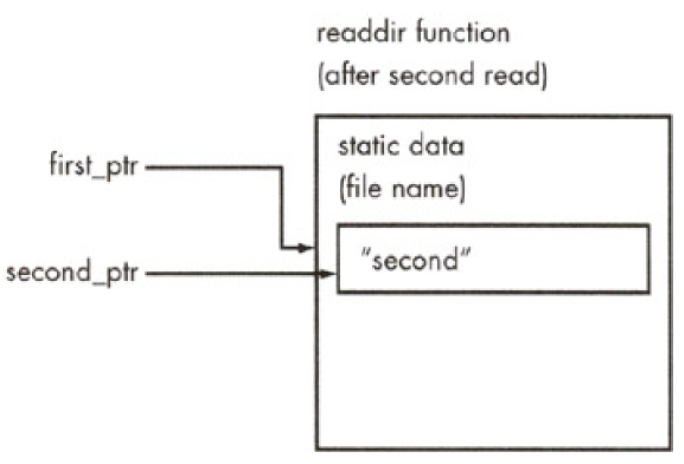
\includegraphics[keepaspectratio,width=0.4\textwidth,height=0.4\textheight]{images/image03.jpg}
\end{center}